\section{Results}
\label{sec:results}

\begin{figure*}[t]
    \centering
    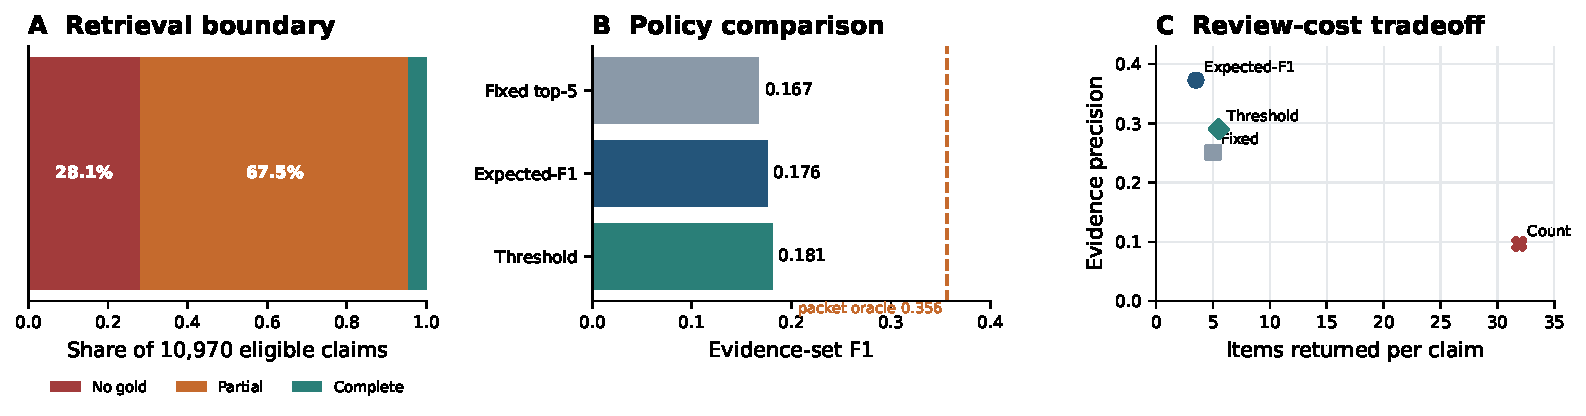
\includegraphics[width=\textwidth]{study_summary.pdf}
    \caption{Study at a glance. (A) Reachability over all 10,970 eligible claims; partial means at least one, but not all, released-gold items are present. (B) Locked-validation evidence F1 of the main policies, where the packet oracle is represented by the dashed boundary. (C) Precision and review-set-size tradeoff.}
    \label{fig:study-summary}
\end{figure*}

\subsection{Retrieval Defines a Low Ceiling}

At the actual operating depths of the selector, complete-gold recall for text is 0.3193 at 40 candidates and for images is 0.2663 at 20 candidates (Table~\ref{tab:operating-retrieval}). The combined packet has an oracle evidence F1 of 0.3560. Among the 10,970 eligible claims, only 4.39\% have all released gold items in the packet, while 3,086 have no reachable gold item. Most claims thus cannot be exactly recovered before set decoding starts.

\begin{table}[t]
\centering
\caption{Retrieval at the packet depths received by every selector.}
\label{tab:operating-retrieval}
\begin{tabular}{lrr}
\toprule
Modality & Retained depth & Complete-gold recall \\
\midrule
Text & 40 & 0.3193 \\
Image & 20 & 0.2663 \\
\bottomrule
\end{tabular}
\end{table}


The expanded retrieval audit also provides a better understanding of what parts are beneficial. Dense-BM25 RRF has a text Recall@50 of 0.3224. When reranking with a cross-encoder, it improves to 0.3338 while early Recall@5 decreases from 0.1772 to 0.1335. For images, SigLIP2-filename RRF achieves Recall@50 of 0.3149, whereas SigLIP2 gets 0.2183 and filename retrieval gets 0.2227. The text reranker sacrifices early ordering for greater recall; image fusion enhances retrieval.

\begin{table*}[t]
\centering
\caption{Complete-gold retrieval quality before packet truncation. Recall includes unretrieved released-gold items in the denominator; MAP and nDCG use the depth-100 ranked lists.}
\label{tab:retrieval-matrix}
\small
\setlength{\tabcolsep}{5pt}
\begin{tabular}{llrrrrrr}
\toprule
Modality & Retriever & R@5 & R@10 & R@20 & R@50 & MAP@100 & nDCG@100 \\
\midrule
Text & Dense sentence & 0.1767 & 0.2141 & 0.2523 & 0.3028 & 0.1728 & 0.2972 \\
Text & BM25 sentence & 0.1452 & 0.1744 & 0.2048 & 0.2478 & 0.1349 & 0.2409 \\
Text & Dense + BM25 RRF & 0.1772 & 0.2194 & 0.2659 & 0.3224 & 0.1744 & 0.3031 \\
Text & RRF + cross-encoder & 0.1335 & 0.1915 & 0.2574 & 0.3338 & 0.1282 & 0.2587 \\
Image & SigLIP2 & 0.1145 & 0.1436 & 0.1782 & 0.2183 & 0.0916 & 0.1312 \\
Image & Filename dense & 0.1408 & 0.1653 & 0.1889 & 0.2227 & 0.1154 & 0.1490 \\
Image & SigLIP2 + filename RRF & 0.1904 & 0.2292 & 0.2663 & 0.3149 & 0.1414 & 0.1938 \\
\bottomrule
\end{tabular}
\end{table*}


As shown in Table~\ref{tab:retrieval-matrix}, the two branches, text and image, fail differently. Text RRF improves both MAP and nDCG over the first-stage models, while the cross-encoder gains deeper Recall@50 at the cost of early precision-sensitive ordering. Image fusion enhances all the reported cutoffs and both ranking metrics, yet its Recall@50 is still below the text branch. This means that a larger packet would contain some evidence that might be missing, but would also reveal a more challenging distractor distribution for the selector.

\begin{table*}[t]
\centering
\caption{Locked-validation performance by packet reachability. The packet oracle selects every reachable released-gold item. Selector values average claim-level F1 across five deterministic training-role partitions.}
\label{tab:reachability-strata}
\begin{tabular}{lrrrrr}
\toprule
Reachability stratum & Claims (share) & Packet oracle & Fixed top-5 & Threshold & Expected-F1 \\
\midrule
No gold reachable & 211 (14.2\%) & 0.000 & 0.000 & 0.000 & 0.000 \\
Partially reachable & 1,200 (80.5\%) & 0.466 & 0.184 & 0.196 & 0.184 \\
Complete gold reachable & 79 (5.3\%) & 1.000 & 0.359 & 0.424 & 0.524 \\
\bottomrule
\end{tabular}
\end{table*}


Table~\ref{tab:reachability-strata} shows how adaptive selection comes in handy in the post hoc validation stratification. For the 79 claims where the entire released-gold set can be obtained, expected-F1 is 0.5240 F1, compared with 0.3593 for fixed top-5 and 0.4237 for thresholding. On the 1,200 partially reachable claims, expected-F1 is 0.1839 and does not improve on fixed top-5 at 0.1841; thresholding is best at 0.1965. The 211 claims where the gold is not reachable have a score of zero for all methods. The aggregate expected-F1 gain is thus localized in the small complete-reachability stratum, while thresholding is more effective for incomplete packets.

\subsection{Prior-Aware Maps Repair Calibration}

Table~\ref{tab:calibration} makes a comparison between maps on locked validation, averaged over modalities and deterministic partitions. Brier scores for identity and temperature are 0.0847 and 0.0832, respectively. They differ by a small amount, consistent with a prior error for which a slope-only temperature is not a cure. Isotonic, Platt and prior-shift calibration further lower the Brier score to around 0.033, and improve the NLL and ECE. When compared to identity calibration, isotonic calibration decreases Brier error by approximately 61\% and ECE from 0.1314 to 0.0063. All five partitions have positive Brier skill relative to the prevalence-only reference, with partition-level skill of roughly 14\%.

\begin{table}[t]
\centering
\caption{Validation calibration averaged across modalities and deterministic partitions.}
\label{tab:calibration}
\begin{tabular}{lrrr}
\toprule
Map & Brier $\downarrow$ & NLL $\downarrow$ & ECE $\downarrow$ \\
\midrule
Isotonic & 0.0330 & 0.1301 & 0.0063 \\
Platt & 0.0331 & 0.1302 & 0.0067 \\
Prior Shift & 0.0331 & 0.1305 & 0.0076 \\
Beta & 0.0359 & 0.3377 & 0.0198 \\
Temperature & 0.0832 & 0.2830 & 0.1220 \\
Identity & 0.0847 & 0.2837 & 0.1314 \\
\bottomrule
\end{tabular}
\end{table}


\begin{figure}[t]
    \centering
    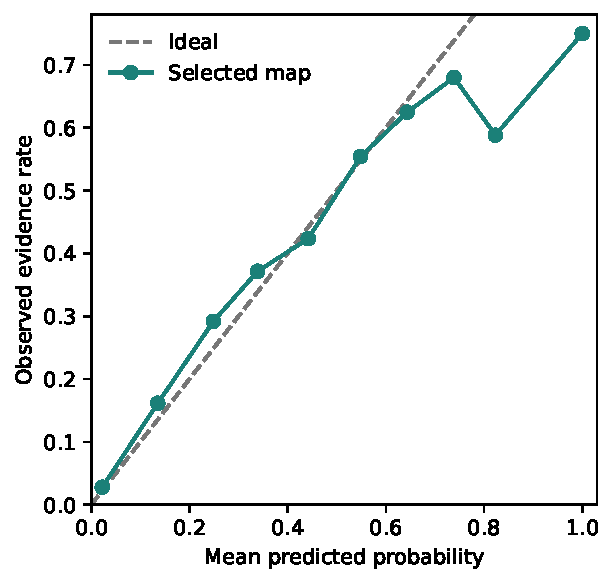
\includegraphics[width=\columnwidth]{calibration_reliability.pdf}
    \caption{Reliability on locked validation. Temperature scaling is still overconfident as it is unable to correct the class-prior shift. Prior-shift, Platt and isotonic maps closely approximate the observed membership rate.}
    \label{fig:calibration}
\end{figure}

Also, after enforcing absolute calibration, scorer choice changes. Partitions 13 and 37 use modality-specific balanced models, while 73 uses an unweighted cross-encoder model, and 101 and 137 use unweighted modality-specific models. For text maps, there is variation between isotonic, Platt and beta maps, while for image scoring, the map is isotonic in all five partitions. This variation may be helpful in considering scorer family, loss weighting, and calibration as a single selection problem.

\subsection{Adaptive Selection Helps, but Thresholding Wins}

The important locked-validation results are shown in Table~\ref{tab:selector-means}. Fixed top-5 reaches 0.1673 evidence F1. Expected-F1 reaches 0.1759 while selecting just 3.50 items per claim. Its precision rises from 0.2511 to 0.3725, while recall falls from 0.1753 to 0.1483. Expected-F1 trades recall for increased precision and a smaller review set.

The highest F1 is achieved by calibrated thresholding, which selects 5.51 items and has an F1 of 0.1807. Learned count prediction selects 31.90 items and gets 0.1100 F1. Without a well-matched set objective, it is not competitive to predict the size.

\begin{table*}[t]
\centering
\caption{Locked-validation evidence-set results over 1,490 claims. Values are means across five deterministic training-role partitions.}
\label{tab:selector-means}
\begin{tabular}{lrrrrr}
\toprule
Method & Precision & Recall & F1 & Exact match & Selected \\
\midrule
Fixed top-5 & 0.2511 & 0.1753 & 0.1673 & 0.0000 & 5.00 \\
Calibrated threshold & 0.2898 & 0.1798 & 0.1807 & 0.0036 & 5.51 \\
Learned count & 0.0965 & 0.2791 & 0.1100 & 0.0001 & 31.90 \\
Expected-F1 & 0.3725 & 0.1483 & 0.1759 & 0.0093 & 3.50 \\
Size-penalized expected-F1 & 0.3725 & 0.1483 & 0.1759 & 0.0093 & 3.50 \\
Size + redundancy expected-F1 & 0.3725 & 0.1483 & 0.1759 & 0.0093 & 3.50 \\
\bottomrule
\end{tabular}
\end{table*}


\begin{table*}[t]
\centering
\caption{Partition-level locked-validation evidence selection. Every row contains the same 1,490 validation claims; partitions change only the training, calibration, and model-selection roles.}
\label{tab:partition-selector-results}
\small
\setlength{\tabcolsep}{5pt}
\begin{tabular}{rrrrrrrr}
\toprule
Partition & Fixed F1 & Threshold F1 & Expected-F1 & Difference & Precision & Recall & Selected \\
\midrule
13 & 0.1677 & 0.1814 & 0.1766 & +0.0089 & 0.3727 & 0.1484 & 3.56 \\
37 & 0.1682 & 0.1811 & 0.1758 & +0.0076 & 0.3774 & 0.1480 & 3.48 \\
73 & 0.1660 & 0.1791 & 0.1761 & +0.0101 & 0.3746 & 0.1476 & 3.43 \\
101 & 0.1674 & 0.1800 & 0.1756 & +0.0082 & 0.3666 & 0.1493 & 3.59 \\
137 & 0.1674 & 0.1818 & 0.1751 & +0.0077 & 0.3714 & 0.1480 & 3.45 \\
\bottomrule
\end{tabular}
\end{table*}


The expected-F1 effect is consistent across the partition-level results in Table~\ref{tab:partition-selector-results}. It has a stable precision-recall profile, a gain of $+0.0076$ to $+0.0101$ over fixed top-5 and a size range of 3.43 to 3.59. The method returns approximately 30\% fewer items on average and improves F1 by approximately 5.1\% relative to fixed top-5. There is no change in the baseline ordering, as thresholding always wins.

The claim-aligned effects in Table~\ref{tab:selector-effects-detail} and Fig.~\ref{fig:selector-effects} confirm these differences. Expected-F1 improves on fixed top-5 by $0.00851$ with a 95\% interval of $[0.00302,0.01400]$ and Holm-adjusted $p=0.0078$. Thresholding improves by $0.01334$ $[0.00931,0.01744]$. Its direct advantage over expected-F1 is $0.00483$ $[0.00003,0.00957]$.

\begin{table}[t]
\centering
\caption{Claim-aligned evidence-F1 effects against fixed top-5.}
\label{tab:selector-effects-detail}
\resizebox{\columnwidth}{!}{%
\begin{tabular}{lrrr}
\toprule
Method & Mean & 95\% interval & Holm $p$ \\
\midrule
Calibrated threshold & +0.0133 & [+0.0093, +0.0174] & 0.0010 \\
Learned count & -0.0574 & [-0.0641, -0.0507] & 0.0010 \\
Expected-F1 & +0.0085 & [+0.0030, +0.0140] & 0.0078 \\
Size-penalized expected-F1 & +0.0085 & [+0.0029, +0.0141] & 0.0078 \\
Size + redundancy expected-F1 & +0.0085 & [+0.0029, +0.0141] & 0.0078 \\
\bottomrule
\end{tabular}%
}
\end{table}


\begin{figure}[t]
    \centering
    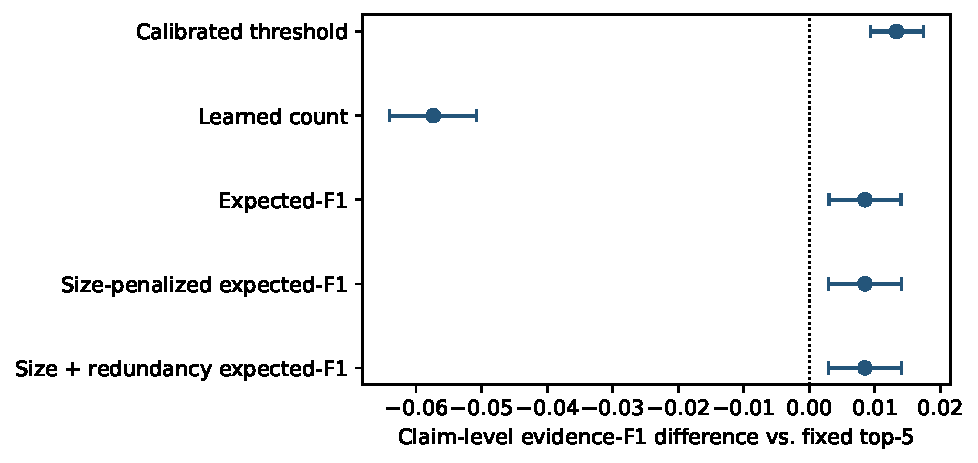
\includegraphics[width=\columnwidth]{corrected_selector_effects.pdf}
    \caption{Claim-aligned evidence-F1 effects with respect to fixed top-5. Points are mean differences and bars are 95\% intervals.}
    \label{fig:selector-effects}
\end{figure}

Both penalty extensions are a perfect match with plain expected-F1. In each partition, the selected size penalty is zero and the selected redundancy penalty is zero. The extra terms introduced complexity without altering the answer on this packet, as can be seen from their claim-level outputs. The quantifiable improvement is through calibrated probabilities.

There is not sufficient evidence to support the superiority condition. Despite the fact that expected-F1 is positive in all partitions and that the corrected interval does not contain zero, it still has a mean gain of 0.00851, which is less than the stated target of 0.015. This experiment therefore provides a small positive development effect, but not enough to surpass the superiority threshold.

\begin{figure*}[!t]
    \centering
    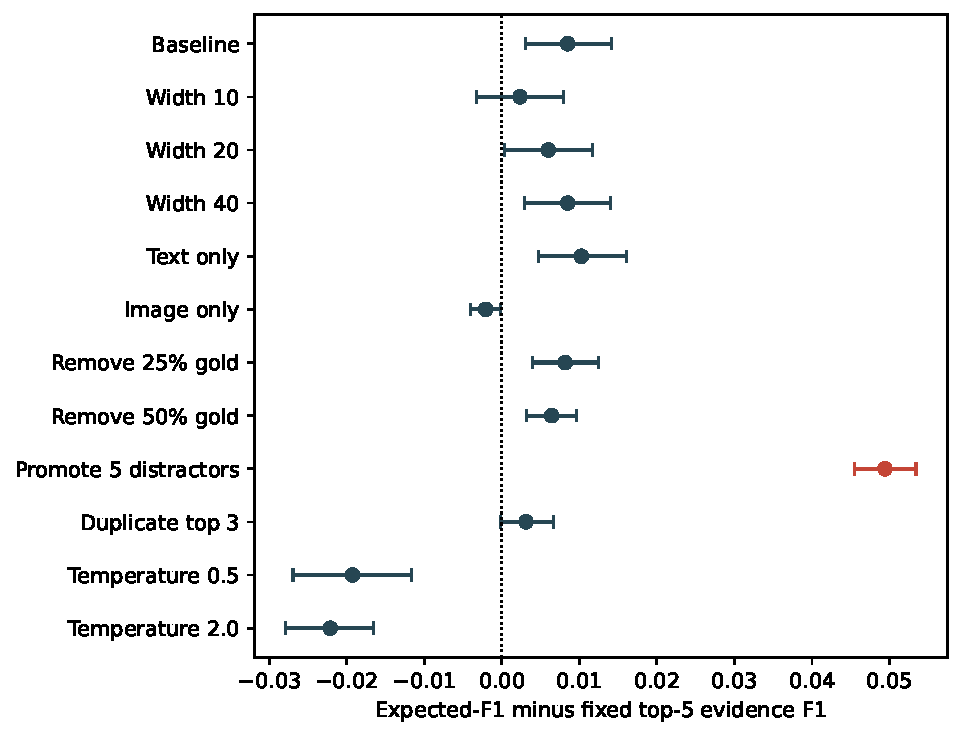
\includegraphics[width=\textwidth]{robustness_effects.pdf}
    \caption{Expected-F1 minus fixed top-5 under controlled perturbations. Probability-temperature changes reverse the baseline gain without changing the candidate ranking.}
    \label{fig:robustness}
\end{figure*}

\subsection{The Verifier Safeguard Remains Unresolved}

We find that the mean difference between expected-F1 and fixed top-5 is $+0.00099$ with a 95\% interval of $[-0.01053,+0.01279]$ under the shared verifier. The lower limit is just below the stated non-inferiority margin of $-0.01$. The point estimate is not far from zero, but the interval does not establish that verdict quality was preserved. Threshold-selected evidence has the highest verifier macro-F1 in every partition (Table~\ref{tab:verifier-effects}).

\begin{table}[t]
\centering
\caption{Shared-verifier macro-F1 by deterministic partition.}
\label{tab:verifier-effects}
\begin{tabular}{lrrrr}
\toprule
Partition & Fixed & Threshold & Expected-F1 & Difference \\
\midrule
13 & 0.3499 & 0.3634 & 0.3472 & -0.0027 \\
37 & 0.3478 & 0.3602 & 0.3525 & +0.0047 \\
73 & 0.3494 & 0.3695 & 0.3488 & -0.0006 \\
101 & 0.3578 & 0.3674 & 0.3579 & +0.0001 \\
137 & 0.3564 & 0.3699 & 0.3598 & +0.0034 \\
\bottomrule
\end{tabular}
\end{table}


\begin{figure}[t]
    \centering
    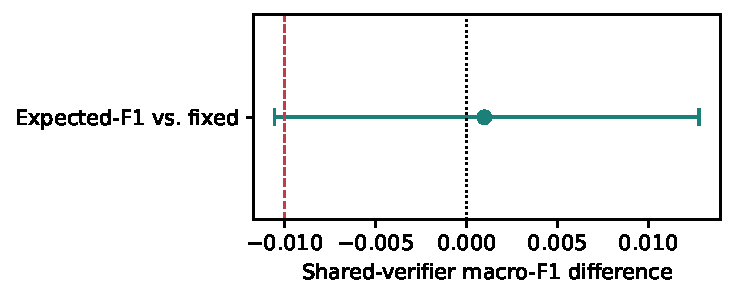
\includegraphics[width=\columnwidth]{corrected_verifier_effect.pdf}
    \caption{Shared-verifier effect of expected-F1 evidence relative to fixed top-5. The $-0.01$ non-inferiority margin is indicated by a dashed line.}
    \label{fig:verifier}
\end{figure}

\subsection{Robustness Exposes Calibration Sensitivity}

There is a positive effect of expected-F1 under width 20 and 40, text-only evidence, and deterministic gold removal. It falls slightly behind fixed top-5 on image-only packets. The impact of promoting five distractors is much bigger because fixed top-5 collapses when all five top positions are filled with distractors; this should not be interpreted as the normal operating impact.

The results are most sensitive to probability perturbations. Sharpening the probabilities with a temperature of 0.5 makes the effect $-0.0193$, and flattening with a temperature of 2.0 makes the effect $-0.0221$. The intervals do not include zero. Expected-F1 is therefore sensitive to probability scale, which does not change candidate order.

Prior-aware maps correct the dominant calibration error and retrieval becomes a hard constraint on the performance that can be achieved. Calibrated expected-F1 offers a slight precision-oriented gain compared to fixed top-5, which is mostly based on claims with full reachable gold. Calibrated thresholding is stronger overall. The advantage depends on probability quality and still does not meet the verifier safeguard.

\clearpage
